\chapter{Linguaggi liberi nondeterministici}
Fino ad ora abbiamo studiato due modi equivalenti per descrivere linguaggi: gli \textbf{automi finiti} e le \textbf{espressioni regolari}. Abbiamo anche visto le limitazioni di questi metodi, che non riescono ad accettare linguaggi, anche alcuni semplici come $ \{0^n 1^n \mid n \geq 0\} $. 

Per espandere la quantita' di linguaggi che possiamo studiare, introduciamo le cosidette \textbf{grammatiche libere (dal contesto)}, un metodo piu' potente che permette di descrivere certe proprieta' di linguaggi che hanno una struttura ricorsiva. Inizialmente queste grammatiche sono state studiate per analizzare linguaggi umani, ma piu' recentemente hanno visto svariate applicazioni, come nel caso dei \textbf{parser}, utilizzati dalla maggior parte di compilatori e interpreti per estrarre il significato dal codice. 

L'insieme dei linguaggi che possono essere riconosciute da grammatiche libere sono i \textbf{linguaggi liberi (dal contesto)}, che includono propriamente i linguaggi regolari. Per riconoscere tali linguaggi, introdurremo un nuovo tipo di automa: l'\textbf{automa a pila} (PDA - pushdown automata).

\section{Grammatiche libere}
Per qualche motivo, le grammatiche libere le abbiamo viste all'inizio, io le metterei qua ma va beh andate qui per capire cosa sono: \ref{dfn: gramLib}

\subsection{Semplificazione e forme normali}
Questa roba qua invece e' stata messa nei linguaggi liberi deterministici, secondo me ha piu' senzo metterla qua' o fare proprio un capitolo solo sulle grammatiche: \ref{semplificazioneGram}

\section{PDA}
In che modo possiamo modificare gli automi visti fin'ora (DFA/NFA) per far si che riescano a riconoscere linguaggi non-regonalari?

Vediamo ad esempio il linguaggio $ L = \{ww^R \mid w \in \{a, b\}^*\} $. Si puo' dimostrare (fallo per esercizio) che non e' un linguaggio regolare, dato che per riconoscerlo si dovrebbe \textbf{memorizzare} tutta la prima parte della parola palindroma (la cui lunghezza non e' limitata). Quindi serve una forma di memoria ausiliaria, che nei PDA e' imlementata con una \textbf{pila} con memoria illimitata. 

Essendo una pila (LIFO), ci sono certe restrizioni per come puo' essere gestita la memoria:
\begin{itemize}
  \item Si puo' leggere solo il primo elemento in cima alla pila (top)
  \item Si puo' rimuovere solo l'elemento top
  \item Si puo' aggiungere elementi solo in cima alla pila (in modo che diventino il nuovo top)
\end{itemize}

I PDA possono essere \textit{nondeterministici}, e come tali hanno una potenza espressiva maggiore rispetto ai PDA deterministici (DPDA). Dimostreremo alla fine della sezione che i PDA (nondeterministici) hanno lo stesso potere espressivo delle grammatiche libere.

\subsection{Definizione formale}
La definizione formale di un PDA e' simile a quella dei NFA, con l'aggiunta della presenza della pila. Questa pila contiene simboli di un alfabeto che puo' essere diverso rispetto a quello di input, quindi dobbiamo definire sia un alfabeto $ \Sigma $ per l'input, sia l'alfabeto $ \Gamma $ per la pila. L'operazione di transizione, che ci dice come si comporta l'automa, ha come dominio $ Q \times \Sigma_\epsilon \times \Gamma $ (dove $ \Sigma_\epsilon = \Sigma \cup \{\epsilon\} $), quindi la mossa del PDA e' determinata dallo stato corrente, dal carattere in input e dal carattere in cima alla pila. Di questi, il secondo puo' essere anche $ \epsilon $, quindi la macchina puo' fare una mossa senza leggere l'input, ma il simbolo in cima alla stack viene sempre letto (e consumato). 

Dato un input, l'automa puo' spostarsi su un nuovo stato e aggiungere un numero arbitrario di elementi alla pila (anche nessuno). Inoltre, dato che il nondeterminismo ha come conseguenza la possibilita' di avere diverse transizioni possibili dato lo stesso input, dobbiamo considerare come codominio l'insieme di tutti i possibili insiemi che hanno come elementi coppie del tipo $ Q \times \Gamma^* $, ovvero l'insieme potenza $ \mathcal{P}(Q \times \Gamma^*) $. 

\dfn{PDA}{
  Un automa a pila nondeterministico e' una 7-pla $ (Q, \Sigma, \Gamma, \delta, q_0, \bot, F) $ dove:
  \begin{itemize}
    \item $ Q $ e' un insieme finito di stati
    \item $ \Sigma $ e' un alfabeto di input finito
    \item $ \Gamma $ e' un alfabeto per la pila finito
    \item $ \delta: Q \times \Sigma_\epsilon \times \Gamma \to Q \times \Gamma^* $ e' la funzione di transizione
    \item $ q_0 $ e' lo stato iniziale
    \item $ \bot \in \Gamma $ e' il primo simbolo sulla pila
    \item $ F \subset Q $ e' l'insieme degli stati finali
  \end{itemize}

}

\subsection{Transizioni}

A ogni passo di computazione, possiamo attribuire a un PDA una \textbf{descrizione instantanea} (o configurazione) che ci dice lo stato corrente $ q \in Q $, l'input rimasto $ w \in \Sigma^* $ e la stringa sulla pila $ \beta \in \Gamma^* $ (dove l'elemento top e' il "carattere piu' a sinistra"): 
\[
(q, w, \beta) 
\]

Le mosse possono essere definite come una derivazione da una configurazione a quella successiva (indicata col simbolo $ \vdash_N $, come con gli altri automi). Mostriamo, usando l'inferenza logica, i due tipi di mossa:
\begin{enumerate}
  \item Lettura di un carattere in input ($ a \in \Sigma $):
    \[
     \frac{(q', \alpha) \in \delta(q, a, X)}{(q, a w, X \beta) \vdash_N (q', w, \alpha \beta)} 
    \]
  \item Senza lettura dell'input:
    \[
      \frac{(q', \alpha) \in \delta(q, \epsilon, X)}{(q, w, X \beta) \vdash_N (q', w, \alpha \beta)}
    \]
\end{enumerate}

Come per gli automi finiti, introduciamo anche $ \vdash^*_N $, la chiusura riflessiva e transitiva di $ \vdash_N $:
\[
  \frac{}{(q, w, \beta) \vdash^*_N (q, w, \beta)} \text{ e } \frac{(q, w, \beta) \vdash^*_N (q', w', \beta') \vdash_N (q'', w'', \beta'')}{(q, w, \beta) \vdash_N (q'', w'', \beta'')}
\]

\subsection{Linguaggio Accettato}
Ci sono diversi modi in cui possiamo determinare se una stringa e' accettata o meno da un PDA. Oltre al classico riconoscimento per stato finale, possiamo dire che una stringa e' accettata se alla fine dell'input la pila e' vuota:
\begin{itemize}
  \item $ L[N] = \{w \in \Sigma^* \mid (q_0, w, \bot) \vdash^*_N (q, \epsilon, \alpha). q \in F\} $
  \item $ P[N] = \{w \in \Sigma^* \mid (q_0, w, \bot) \vdash^*_N (q, \epsilon, \epsilon)\} $
\end{itemize}

Osserviamo che non per forza un PDA deve svuotare la pila alla fine di un input accettato, quindi in generale:
\[
  L[N] \neq P[N]
\]
Dimostriamo pero' che questi due metodi di riconoscimento hanno la stessa espressivita':
\thm{}{
  Dato un PDA $ N $ si ha che:
  \begin{itemize}
    \item Se $ L = L[N] $ e' il linguaggio riconosciuto da $ N $ per stato finale, allora $ \exists N' $ PDA tale che $ L = P[N'] $, dove $ P[N'] $ e' il linguaggio riconociuto da $ N' $ per pila vuota.
    \item Viceversa, se $ L = P[N] $ allora $ \exists N'' $ PDA tale che $ L = L[N''] $.
  \end{itemize}
  Quindi i PDA che riconoscono per stato finale e quelli che riconoscono per pila vuota sono equivalenti.
}
Vediamo prima un'osservazione che ci servira' per dimostrare questo teorema:
\nt{
  Si osservi che, se la pila viene completamente svuotata, il PDA che abbiamo definito non puo' avere altre transizioni. Questo e' perche' $ \epsilon \not\in \Gamma $, e quindi non e' neanche presente nel dominio della funzione di transizione. Quindi se la pila di un PDA e' vuota, allora si blocca.
}
Detto questo, passiamo a una dimostrazione per costruzione di entrambe gli enunciati: TODO aggiungi figure
\pf{Dimostrazione}{
  Dimostriamo (in ordine inverso) i due versi:
  \begin{itemize}
    \item Sia $ N $ un PDA che accetta un linguaggio $ L $ per pila vuota ($ L = P[N] $). Costruiamo un PDA $ N' $ che riconosca lo stesso linguaggio per stato finale. L'idea e' quella di aggiungere un elemento in fondo alla pila, in modo tale da poter riconoscere quando la pila di $ N $ si sarebbe svotata, e di aggiungere transizioni da tutti gli stati ad un nuovo stato finale. Per aggiungere l'elemento sulla pila, basta aggiungere un nuovo stato iniziale con una transizione verso il vecchio stato iniziale che non legga l'input e che aggiunga un elemento $ Z \not\in \Gamma $ sotto a $ \bot $. 

      Le  transizioni aggiuntive non leggono caratteri in input (sono nondeterministiche) e guardano se in cima alla pila e' presente l'elemento finale aggiunto inizialmente. In questo modo, se la pila non arriva mai all'ultimo elemento allora e' impossibile arrivare allo stato finale, mentre se la pila viene svuotata e' possibile spostarsi sullo stato finale. Se $ N' $ si trova nell'ultimo caso ma non ha finito di leggere la stringa, il PDA si blocca e la parola non viene accettata. Altrimenti viene riconosciuta, sse appartiene al linguaggio $ L $.
    \item Sia $ N $ un PDA che accetta un linguaggio $ L $ per stato finale ($ L = L[N] $). Costruiamo un PDA $ N'' $ che riconosca lo stesso linguaggio per pila vuota. L' idea e' simile a quella sopra: aggiungiamo un elemento $ Z \not\in \Gamma $ in fondo alla pila (sempre per evitare che la pila si svuoti, rendendo impossibili ulteriori transizioni), e aggiungiamo delle transizioni nondeterministiche, questa volta solo dagli stati finali di $ N $, che portano a uno stato da cui parte un'unica transizione verso se stesso. Questa transizione non fa altro che rimuovere elementi dalla pila senza leggere input, in modo che se $ N $ arriva ad uno stato finale dopo aver conumato tutto l'input, allora $ N'' $ ha una possibile strada che svuota completamente la pila. Altrimenti, o la pila non viene mai svuotata, oppure viene svotata ma senza consumare tutto l'input (e quindi non viene riconosciuta). Osservare che in tutte le altre transizioni non si puo' leggere $ Z $ dalla pila (dato che non appartiene all'alfabeto della pila), quindi non potra' accadere che la pila si svuoti consumando tutto l'input senza raggiungere lo stato aggiunto, riconoscendo erroneamente l'input.
  \end{itemize}
}

\section{Equivalenza fra grammatiche libere e PDA}
In questa sezione dimostreremo che i PDA e le grammatiche libere hanno lo stesso potere espressivo, ovvero che riconoscono lo stesso insieme di linguaggi. Quindi sia le grammatiche libere che i PDA riconoscono linguaggi liberi e faremo vedere come costruire un PDA equivalente partendo da una CFG (context free grammar) e viceversa. Dato che per definizione un linguaggio e' libero sse esiste una grammatica libera che lo descrive, ci riduciamo a dimostrare il seguente teorema:
\thm{}{
  Un linguaggio e' libero sse esiste un PDA che lo riconosce
}

Dobbiamo dimostrare le due direzioni. Dato che sono un po' corpose, separiamole in due lemmi:
\subsection{Da grammatica libera a PDA}
\mlenma{}{
  Dato un linguaggio libero $ L $, esiste un PDA $ N $ tale che 
  \[
    L = P[N]
  \]
}
Notare che potevamo anche scrivere $ L = L[N] $, dato che abbiamo dimostrato che i due metodi di riconoscimento hanno la stessa espressivita'. Per la dimostrazione ci e' piu' utile costruire un PDA che riconosca per pila vuota, andiamo a vedere come costruirlo:
\pf{Idea della dimostrazione}{
  Data la grammatica libera $ G $ che descrive $ L $, vogliamo costruire un PDA $ N $ che accetta un input $ w $ se esiste una derivazione di $ G $ che porta a $ w $. Ricordiamo che una derivazione e' la serie di sostituzioni che fa una grammatica, partendo dalla variabile iniziale, per generare una stringa. Ad ogni passo viene generata una \textbf{stringa intermedia} formata da terminali e non-terminali. Il compito di $ N $ e' quello di decidere se esistono una serie di sostituzioni (prese dalle regole di $ G $) che generano $ w $.

  La parte difficile e' sapere quale sostituzione e' quella giusta, dato che possono esserci piu' regole di sostituzione per una sola variabile. Fortunatamente, utilizzando il nondeterminismo possiamo semplicemente considerare tutte le opzioni come percorsi validi. 

  Allo stato iniziale, quindi, il PDA si ritrova solo il nonterminale $ S $ sulla pila. Poi passa per una serie di stringhe intermedie prima di avere solo terminali, che se combaciano con l'input significa che esiste una derivazione di $ G $ che genera $ w $ e quindi $ N $ lo accetta. Se in tutte le possibili diramazioni nondeterministiche l'input non combacia con la stringa nella pila, allora $ G $ non puo' generarlo e non viene riconosciuto da $ N $. 

  L'unico problema e' che un PDA puo' solo accedere al primo elemento della pila. Questo significa che se un non-terminale non e' top, non possiamo sostituirlo senza rimuovere tutti i terminali sopra, quindi non possiamo tenere in memoria l'intera stringa intermedia. Possiamo risolvere questo problema consumando il top ogni volta che appare un terminale che combacia con il carattere in input, passando quindi al carattere successivo. Se non combaciano, il PDA deve fare \textit{backtracking} e provare una nuova combinazione di sostituzioni. Se per tutte le combinazioni c'e' un terminale in top che non combacia con l'input, la stringa non viene accettata. 

  Notare che in questo modo, il PDA svolge una \textbf{derivazione leftmost} (\ref{dfn: derLeft}) dal simbolo iniziale all'input.
}
\pf{Dimostrazione formale}{
  Sia $ L $ un linguaggio libero. Allora per definizione esiste una grammatica $ G = (NT, T, R, S) $ che lo descrive. Vogliamo costruire un PDA $ N $ tale che $ L = P[N] $. Sia $ N = (\{q\}, T, NT \cup T, \delta, q, S, \emptyset) $. Aggiungiamo le transizioni $ \forall a \in T $, $ \forall A \in NT $:
    \begin{align*}
      \delta(q, a, a) &= \{(q, \epsilon)\}\\
      \delta(q, \epsilon, A) &= \{(q, \beta) \mid A \to \beta \in R\}
    \end{align*}
  Si puo' dimostrare per induzione sulla lunghezza dell'input che:
  \[
    S \Rightarrow_l^* w \iff (q, w, s) \vdash_N^* (q, \epsilon, \epsilon) 
  \]
}

\subsection{Da PDA a grammatica libera}
\mlenma{}{
  Dato un PDA $ N $ tale che $ L = P[N] $, possiamo costruire una grammatica libera $ G $ tale che:
  \[
    L = L[G]
  \]
}
Questa direzione e' molto piu' lunga e complessa rispetto alla prima, dato che "programmare" un automa e' molto piu' semplice rispetto a "programmare" una grammatica. E piu' semplice dimostrare il lemma se consideriamo un PDA con un solo stato, quindi ci torna utile il seguente lemma:
\mlenma{}{
  Per ogni PDA $ N $, esiste un PDA $ N' $ con un solo stato tale che:
  \[
    P[N] = P[N']
  \]
}
Questo lemma ci dice che ogni PDA puo' essere trasformato in un PDA equivalente che ha un solo stato. Non lo dimostriamo perche sbattecazz.

Ora ci possiamo ricondurre a dimostrare il lemma con l'ipotesi aggiuntiva che $ N $ ha un solo stato:
\pf{Idea della dimostrazione}{
  Dato che la dimostrazione formale e' davvero lunghissima, tale da mandare in tilt anche il dio degli audiolibri detto "Il Guerriero", ne parleremo solo schematicamente.

  L'idea e' la seguente: dato un PDA $ N = (\{q\}, \Sigma, \Gamma, \delta, q, \emptyset) $ a uno stato, generiamo una grammatica libera $ G = (T, NT, R, S) $ equivalente tale che:
  \begin{align*}
    \forall a \in \Sigma_\epsilon, \forall A \in \Gamma. & (q, B_1B_2...B_k)  \in \delta(q, a, A) \text{ con } k \geq 0:\\
    & A \to aB_1B_2...B_k \in R
  \end{align*}

  Si puo' dimostrare che $ S \Rightarrow^* w \iff (q, w, s) \vdash_N^* (q, \epsilon, \epsilon) $.
}
\subsection{Relazione fra linguaggi regolari e linguaggi liberi}
Abbiamo quindi dimostrato che gli automi a pila riconoscono la classe di linguaggi liberi. Dato che gli automi finiti riconoscono i linguaggi regolari e possono essere convertiti in PDA che ignorano la pila, possiamo dire che:
\mprop{Relazione fra linguaggi regolari e linguaggi liberi}{
  I linguaggi regolari sono un sottoinsime proprio dei linguaggi liberi.
}
TODO: figura

\section{Proprieta'}
\subsection{Chiusura}
Come nei linguaggi regolari, anche i linguaggi liberi sono chiusi rispetto alle operazioni regolari:
\thm{}{
  I linguaggi liberi sono chiusi per:
  \begin{enumerate}
    \item Unione
    \item Concatenazione
    \item Ripetizione (stella di Kleene)
  \end{enumerate}
}
\pf{Dimostrazione}{
  Siano $ L_1, L_2 $ i linguaggi generati da due grammatiche libere $ G_1 = (NT_1, T_1, R_1, S_1), G_2 = (NT_2, T_2, R_2, S_2) $ e assumiamo che $ NT_1 \cap NT_2 = \emptyset $, allora:
  \begin{enumerate}
    \item \textbf{Unione:}

      Costruisco la grammatica libera $ G = (NT_1 \cup NT_2 \cup \{S\}, T_1 \cup T_2, R_1 \cup R_2 \cup \{S \to S_1 \mid S_2\}, S) $. Si puo' dimostrare che $ L(G) = L_1 \cup L_2 $.

    \item \textbf{Concatenazione:}

      Costruisco la grammatica libera $ G = (NT_1 \cup NT_2 \cup \{S\}, T_1 \cup T_2, R_1 \cup R_2 \cup \{S \to S_1S_2\}, S) $. Si puo' dimostrare che $ L(G) = L_1 \cdot L_2 $.

    \item \textbf{Ripetizione:}

      Costruisco la grammatica libera $ G = (NT_1 \cup \{S\}, T_1, R_1 \cup \{S \to \epsilon \mid S_1S\}, S) $. Si puo' dimostrare che $ L(G) = L_1^* $.
  \end{enumerate}
}
Rispetto all'intersezione:
\thm{}{
  Dati un linguaggio libero $ L_1 $ e un linguaggio regolare $ L_2 $, la loro intersezione $ L_1 \cap L_2 $ e' un liguaggio libero.
}
Notare che questo teorema \textbf{NON} dice che i linguaggi liberi sono chiusi rispetto all'intersezione (infatti vedremo dopo che non lo sono). Dimostriamolo:
\pf{Idea della dimostrazione}{
  Vogliamo in qualche modo eseguire contemporaneamente sia il PDA che riconosce il linguaggio libero (per stato finale), sia il DFA che riconosce il linguaggio regolare. Se alla fine dell'input sono entrambe in stato di riconoscimento, allora significa che la stringa fa parte sia del linguaggio regolare che di quello libero, quindi appartiene all'intersezione.
}
\pf{Dimostrazione}{
  Dati un PDA $ N_1 = (Q_1, \Sigma, \Gamma, \delta_1, q_1, Z, F_1) $ e un DFA $ N_2 = (Q_2, \Sigma, \delta_2, q_2, F_2) $ che riconoscono rispettivamente il linguaggio libero $ L_1 = L[N_1] $ e il linguaggio regolare $ L_2 = L[N_2] $, costruiamo un PDA $ N $ che riconosca il linguaggio $ L_1 \cap L_2 $:
   \begin{itemize}
      \item $ N = (Q_1 \times Q_2, \Sigma, \Gamma, \delta, \innerproduct{q_1}{q_2}, Z, F_1 \times F_2) $
      \item $ \forall q \in Q_1, \forall p \in Q_2,\forall a \in \Sigma,\forall X \in \Gamma: $
        \[
          \delta(\innerproduct{q}{p}, a, X) = \{(\innerproduct{r}{s}, \gamma) \mid s = \delta_2(p, a) \land \innerproduct{r}{\gamma} \in \delta_1(q, a, X)\}
        \]
   \end{itemize}
   Si puo' dimostrare che $ \forall w \in \Sigma^* $:
   \[
     (q_1, w, Z) \vdash_{N_1}^* (q, \epsilon, \gamma) \land \hat{\delta}_2(q_2, w) = q'
   \]
   \begin{center}
     sse
   \end{center}
   \[
     (\innerproduct{q_1}{q_2}, w, Z) \vdash_N^* (\innerproduct{q}{q'}, \epsilon, \gamma)
   \]
   Quindi, se $ q \in F_1 $ e $ q' \in F_2 $ e quindi $ w \in L_1 \cap L_2 $, anche $ N $ riconosce $ w $ dato che $ \innerproduct{q}{q'} \in F_1 \times F_2 $. Vale anche la direzione opposta, quindi $ L_1 \cap L_2 = L[N] $. 
}
Possiamo usare questa proprieta' per dimostrare che un linguaggio non e' libero. Infatti, dato un linguaggio $ L_1 $ che vogliamo analizzare, basta trovare un linguaggio $ L_2 $ regolare per cui $ L_1 \cap L_2 $ non e' libero. Se riusciamo a trovare tale linguaggio, allora siamo sicuri che $ L_1 $ non e' regolare:
  \begin{align*}
    & \forall L_1, \\
    & \exists L_2 \text{ regolare } L_1 \cap L_2 \text{ non e' libero} \implies L_1 \text{ non e' libero}
  \end{align*}

I linguaggi liberi, come anticipato, non sono chiusi per intersezione. Per dimostrarlo, basta trovare una controprova:
\pf{Controprova}{
  Consideriamo i due linguaggi liberi $ L_1 = \{a^nb^nc^m \mid n,m\geq 0\} $ e $ L_2 = \{a^nb^mc^m \mid n,m\geq 0\} $. Le uniche stringhe che appartengono sia a $ L_1 $ che a $ L_2 $ sono quelle che hanno lo stesso numero di tutti e tre i caratteri, ovvero: $ L_1 \cap L_2 = \{a^nb^nc^n \mid n\geq 0\} $. Vediamo ora il \textbf{pumping thorem} per dimostrare che questo linguaggio non e' libero.
}
\subsection{Pumping Theorem}
Il \textbf{pumping theorem} ci serve per dimostrare qundo linguaggio non fa parte della classe di linguaggi liberi. Si ricordi il pumping lemma (TODO: aggiungi ref), introdotto con i linguaggi regolari. Il pumping theorem e' abbastanza simile, dato che anche questo dimostra l'esistenza di una \textbf{lunghezza di pompaggio} per i linguaggi liberi, tale che ogni stringa di lunghezza maggiore o uguale puo' essere pompata. In questo caso, pero', non c'e' una sola sezione che puo' essere ripetuta, ma due. Vediamo in dettaglio:
\thm{}{
  Se $ L $ e' un linguaggio libero, allora esiste un numero $ p $ tale che, sia $ s \in L $ con $ |s| \geq p $, allora $ s $ puo' essere divisa in cinque sezioni $ s = uvxyz $ che soddisfano tali condizioni:
  \begin{enumerate}
    \item $ \forall i \geq 0, uv^ixy^iz \in L $
    \item $ |vy| > 0 $
    \item $ |vxy| \leq p $
  \end{enumerate}
}
La seconda condizione ci dice che $ v $ o $ y $ devono essere non nulli, se no il teorema diventa ovviamente vero per ogni linguaggio. La terza condizione ci puo' aiutare in alcune dimostrazioni.
\pf{Idea della dimostrazione}{
  Per capire questa dimostrazione, e' necessario avere ben presente le grammatiche libere e i relativi alberi di derivazione (\ref{dfn: alberoDer}). Infatti dato che $ L $ e' un linguaggio libero, avra' anche una grammatica che lo genera. 

  Consideriamo una parola $ s \in L $ "abbastanza lunga" (defineremo dopo cosa significa): questa avra' almeno un'\textbf{albero di derivazione} che la genera. Avendo scelto $ s $ abbastanza lunga, allora la distanza massima dalla radice $ S $ a una foglia (ovvero l'\textbf{altezza dell'albero}) e' tale da garantire, per il \textbf{pigeonhole principle}, il ripetersi di uno dei nonterminali fra i nodi del percorso.

  Chiamiamo $ A $ il nonterminale ripetuto. Come si vede dalla figura, possiamo rimpiazzare il sottoalbero radicato nella seconda ripetizione di $ A $ con il sottoalbero radicato nella prima ripetizione di $ A $, ottenendo un albero di derivazione valido e quindi una stringa appartenente a $ L $. Possiamo ripetere questa procedura all' infinito, e vale anche se facciamo al contrario.

  Quindi, se divido $ s $ in cinque sezioni $ uvxyz $ come indica la figura, e' possibile ripetere $ v $ e $ y $ e ottenere sempre parole che appartengono a $ L $.

\begin{center}
  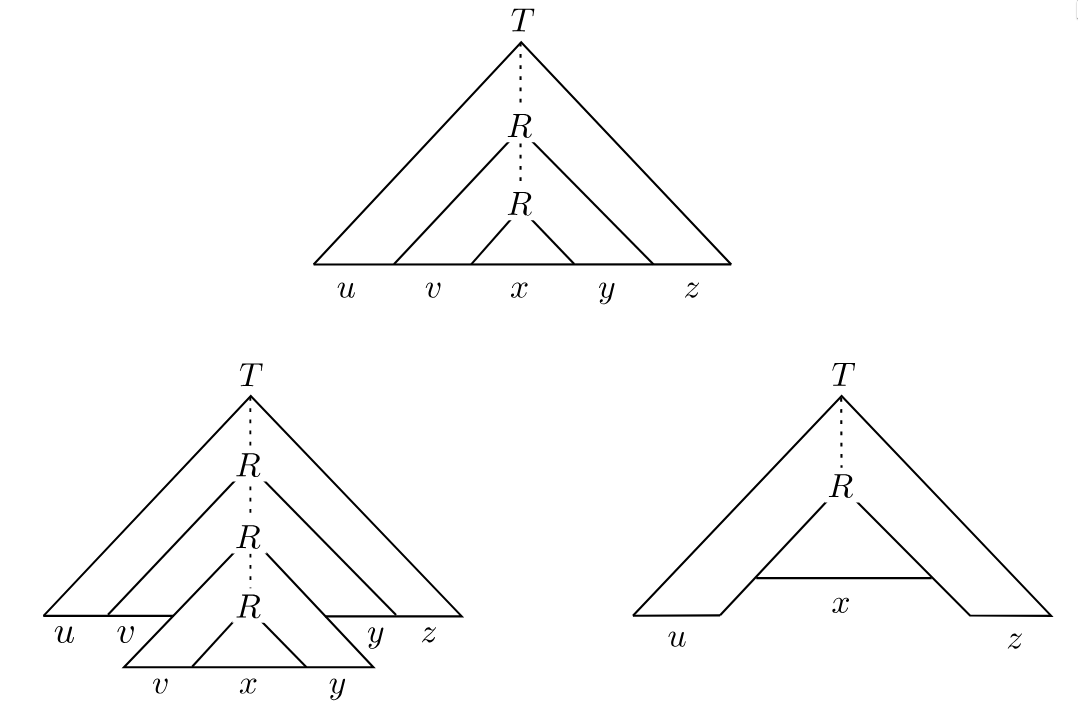
\includegraphics[scale=0.3]{img/2024-12-07-18-52-41.png}
\end{center}

}

Entriamo ora nei dettagli e proviamo a dimostrare in modo piu' formale tutte e tre le condizioni, oltre a vedere come calcolare la lunghezza di pompaggio $ p $:
\pf{Dimostrazione}{
  Sia $ G = (T, NT, R, S) $ una grammatica libera che genera $ L $. Sia $ b $ il massimo numero di simboli (sia $ T $ che $ NT $) che si trovano nella parte destra di una produzione in $ R $ ($ b = max \{|\alpha| \mid A \to \alpha \in R\} $). Possiamo assumere che $ b \geq 2 $, dato che altrimenti la grammatica sarebbe banale. In qualsiasi albero di derivazione generato da $ G $, il massimo numero di figli che puo' avere un nodo e' $ b $. In altre parole, ci saranno un massimo di $ b $ nodi che distano $ 1 $ dalla radice $ S $, al massimo $ b^2 $ che distano $ 2 $ e in generale un massimo di $ b^h $ nodi che distano esattamente $ h $ dalla radice. Quindi, se un albero e' alto $ h $ la stringa che genera e' lunga al massimo $ b^h $. Viceversa, se una stringa e' lunga almeno $ b^h + 1 $, allora il suo albero di derivazione sara' alto almeno $ h+1 $.
  \[
    |w| \geq b^h + 1 \implies \text{height(parseTree(w))} \geq h+1
  \]
  Sia $ |NT| $ il numero di nonterminali in $ G $, impostiamo la lunghezza di pompaggio nel seguente modo: $ p = b^{|NT|+1} $. Dato che $ b \geq 2 $, sappiamo che $ p > b^{|NT|} $, e quindi $ p \geq b^{|NT|}+1 $ (tecnicamente si puo' mettere maggiore stretto, ma per la dimostrazione non serve). Cosi' facendo, se $ s $ e' una stringa di $ L $ tale che $ |s| \geq p $, sappiamo che il suo albero di derivazione e' alto almeno $ |NT|+1 $:
  \[
    |w| \geq p = b^{|NT|+1} \geq b^{|NT|}+1 \implies \text{height(parseTree(w))} \geq |NT|+1
  \]
Notare che l'implicazione vale anche se poniamo $ b^{|NT|}+1 $ come pumping length, ma per garantire la terza condizione dobbiamo scegliere la lunghezza maggiore che puo' generare un albero alto $ |NT|+1 $, vedremo dopo perche'.

Per vedere come pompare una stringa $ w \in L, |w| \geq p $, chiamiamo $ \tau $ il suo albero di derivazione che ha il minor numero di nodi (questa condizione serve per garantire la seconda condizione). Sappiamo che $ \text{heigth}(\tau) \geq |NT|+1 $, ovvero che esiste un percorso dalla radice a una foglia lungo almeno $ |NT|+1 $. Contando la radice, ci sono $ |NT|+2 $ nodi lungo questo percorso, di cui uno e' la foglia che e' quindi un terminale. Quindi i restanti $ |NT| + 1 $ nodi sono tutti nonterminali, e per il \textit{pigeonhole principle} almeno uno si deve ripetere. Chiamiamo $ A $ il nonterminale che si ripete entro i $ |NT|+1 $ nonterminali "piu' in basso", ovvero piu' vicini alla foglia, lungo il percorso (questa scelta serve per garantire la terza condizione).

Dividiamo $ w $ in cinque parti $ uvxyz $ come nella figura. L' occorrenza superiore di $ A $ ha un sottoalbero piu' grande che genera $ vxy $, mentre quella piu' in basso ha un sottoalbero piu' piccolo e genera solo $ x $. Entrambe le sottostringhe sono generate dalla stessa variabile, quindi possiamo sostituire l'una con l'altra e ottenere un nuovo albero di derivazione valido. Sostituendo il minore con il maggiore ripetutamente ci da tutti gli alberi di derivazione per le stringhe $ uv^ixy^iz $ con $ i > 1 $. Sostituendo il maggiore con il minore otteniamo la stringa $ uxz $ (il caso in cui $ i = 0 $), quindi abbiamo stabilito che questa divisione soddisfa la prima condizione, vediamo le altre due:

Per la condizione 2, dobbiamo accertarci che $ u $ e $ y $ non siano entrambe $ \epsilon $. Usando l'eliminazione del not, assumiamo che siano entrambe $ \epsilon $ e dimostriamo il falso. Se fosse cosi', potremmo sostituire il sottalbero minore a quello maggiore ottenendo comunque la stringa iniziale ($ uxz = uv^ixy^iz $), pero' con un albero piu' piccolo. Ma questo e' assurdo, perche' come ipotesi avevamo stabilito che $ \tau $ fosse l'albero di derivazione di $ w $ con meno nodi. 

La terza condizione dice che $ |vxy| \leq p $. Questa e' la sottostringa generata dalla prima occorrenza di $ A $ (dalla radice verso le foglie), il cui sottoalbero e' alto al massimo $ |NT| + 1 $, dato che le due ripetizioni di $ A $ devono essere entro i $ |NT|+1 $ nonterminali piu' vicini alla foglia. La stringa piu' lunga che puo' generare un albero di quell'altezza e' $ b^{|NT|+1} = p $, quindi $ |vxy| \leq p $ come volevamo dimostrare.
}

